
\section{Aplicaci�n de Data Discovery a datos de instituciones del Estado}

\begingroup
\setlength{\intextsep}{-20pt}%
\setlength{\columnsep}{5pt}%
\begin{wrapfigure}{r}{0.25\textwidth}
	\centering
	
\includegraphics[width=\linewidth]{figuras/makeDecision}
	\vspace{-10pt}
	\caption{}
	\label{fig:makeDecision}
\end{wrapfigure}
En Paraguay, e inclusive mundialmente, la mayor�a de las empresas no logran comprender 100\% los datos que generan. La consecuencia de no comprender los datos puede conllevar a tomar una decisi�n equivocada y esa decisi�n puede terminar en algo irreversible y de mucho impacto negativo para la organizaci�n a lo largo del tiempo. La informaci�n es considerada como uno de los recursos m�s importantes en una empresa, porque en base a esto se obtiene el conocimiento.

Aplicando la t�cnica de data discovery podremos detectar irregularidades, predecir acontecimientos futuros y preverlos a tiempo. En este trabajo analizaremos los datos de la ANDE y de la DGEEC, realizando cruzamiento entre ambos, con el objetivo de obtener informaci�n de inter�s para la entidad.
\endgroup 

\subsubsection{Datos de la ANDE y de la DGEEC}

Se cuenta con datos de consumo de energ�a el�ctrica, importe facturado, grupo de consumo (residencial, industrial, exportaci�n, etc), por a�o (2000-2014), departamento y distrito. Estos datos fueron solicitados formalmente a la entidad a trav�s de la Facultad de Ciencias y tecnolog�a de la Universidad Cat�lica, la cual tuvimos una respuesta favorable para proceder.

\subsubsection{Dashboard de control / monitoramiento}
	
En esta secci�n se mostrar�n 4 ejemplos de paneles hechos con los datos de ambas instituciones (DGEEC y ANDE).  Una de las t�cnicas de comparaci�n a ser utilizadas en los gr�ficos es ,  ``Medici�n de tasas de crecimientos``, la cual se calcula el porcentaje de crecimiento que hubo por cada a�o. Por ejemplo, si al cerrar el a�o 2014, la cantidad de clientes lleg� a 1.000.000 y en el a�o 2015 aument� 100.000, esto quiere decir que en el a�o 2015, la tasa de crecimiento de los clientes fue del 10\%, es decir, hubo un crecimiento positivo y la cantidad de clientes ha aumentado el respecto al a�o anterior. Suponiendo que el a�o 2016 la ANDE cierra con un total de 1.000.000 clientes,, su crecimiento ser� de 10\% negativo.
La f�rmula empleada es la que sigue, donde ``n`` es el a�o actual y ``n-1`` el a�o anterior, PIB es una variable que indica, en el caso  de nuestra comparaci�n, la cantidad de clientes que posee la ANDE .
	
\textsc{\begin{figure}[H]
	\centering
	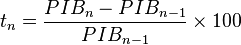
\includegraphics[width=0.7\linewidth]{figuras/formula}
	\caption{Form�la para hallar taza de crecimiento.}
	\label{fig:formula}
\end{figure}}
	
\subsection{Dashboard - Clientes Facturados vs Crecimiento Poblacional}
Este dashboard se realiz� a fin de cruzar los datos del DGEEC y la ANDE, se utilizan datos hist�ricos de la poblaci�n y datos de clientes, consumo e importe de la ANDE.

\textsc{\begin{figure}[H]
	\centering
	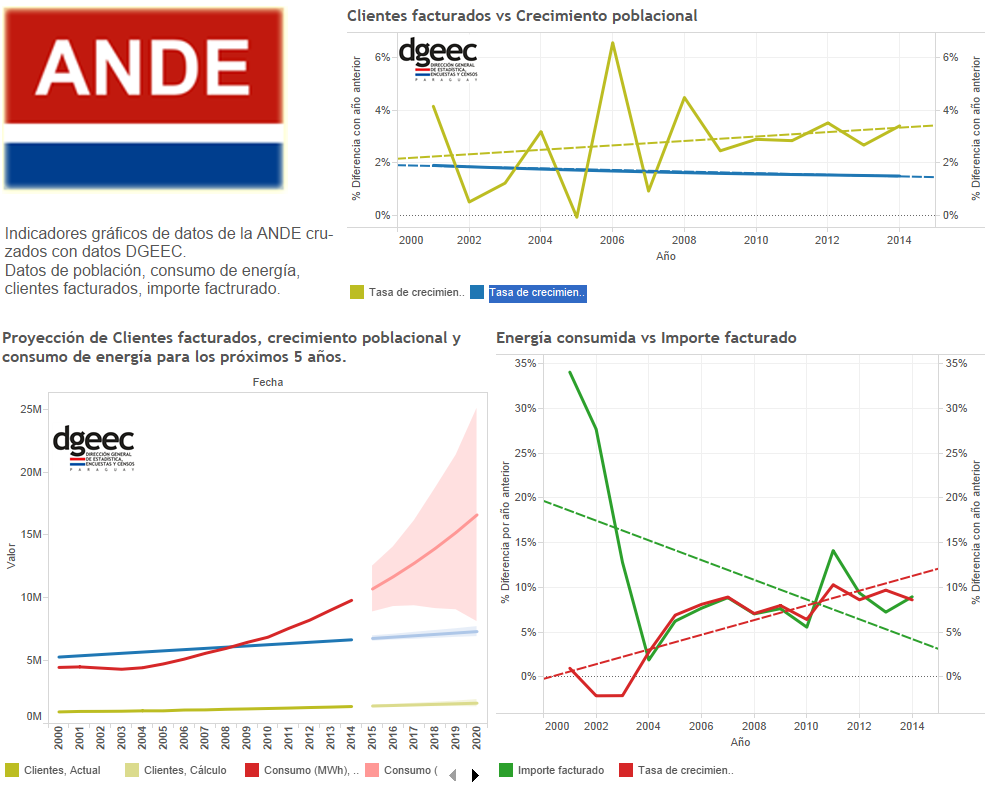
\includegraphics[width=\linewidth]{figuras/ClientesFacturadosVsCrecimientoPoblacional3}
	\caption{Clientes Facturados vs Crecimiento Poblacional}
	\label{fig:ClientesFacturadosVsCrecimientoPoblacional3}
\end{figure}}

El siguiente gr�fico representa el porcentaje del crecimiento anual de los clientes en comparaci�n con el de la poblaci�n. Podemos observar que la l�nea que pertenece a la tasa de crecimiento de la poblaci�n (azul), fue bajando al pasar los a�os. Esto no quiere decir que la poblaci�n fue disminuyendo, sino que cada a�o el porcentaje de aumento es menor.

\textsc{\begin{figure}[H]
	\centering
	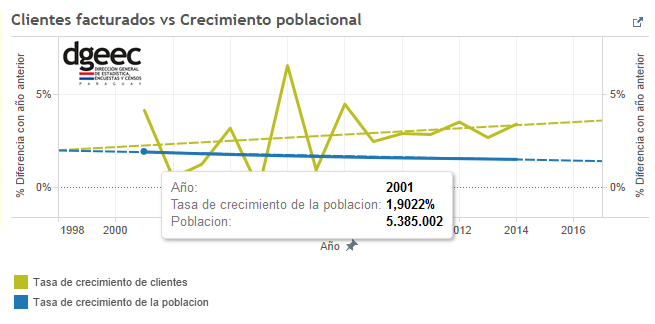
\includegraphics[width=\linewidth]{figuras/ClientesFacturadosVsCrecimientoPoblacional4}
	\caption{Clientes Facturados vs Crecimiento Poblacional}
	\label{fig:ClientesFacturadosVsCrecimientoPoblacional4}
\end{figure}}


\textsc{\begin{figure}[H]
	\centering
	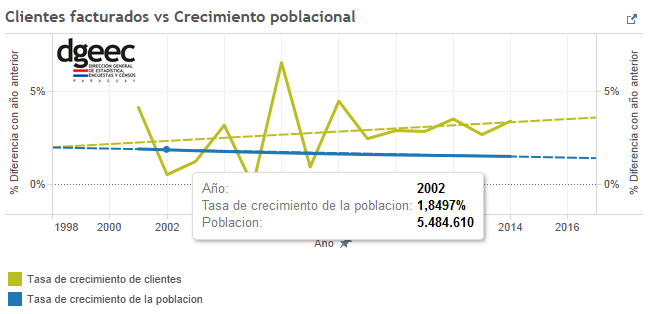
\includegraphics[width=\linewidth]{figuras/ClientesFacturadosVsCrecimientoPoblacional}
	\caption{Clientes Facturados vs Crecimiento Poblacional}
	\label{fig:ClientesFacturadosVsCrecimientoPoblacional}
\end{figure}}

La l�nea amarilla representa al porcentaje del crecimiento de los clientes de la ANDE. Como podemos ver, hay      a�os en que el aumento es muy notorio (2004,2006,2008) y hay a�os en que este es m�nimo(2002,2005,2007). Las l�neas discontinuas representan las tendencias de ambos puntos. Por ejemplo, la cantidad de clientes en el a�o 2001 fue de 959.580, la cual aument� el 4.1\% respecto al a�o anterior. 

\textsc{\begin{figure}[H]
	\centering
	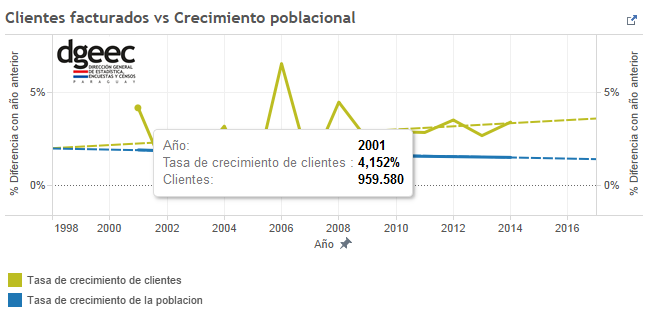
\includegraphics[width=\linewidth]{figuras/ClientesFacturadosVsCrecimientoPoblacional2}
	\caption{Clientes Facturados vs Crecimiento Poblacional}
	\label{fig:ClientesFacturadosVsCrecimientoPoblacional2}
\end{figure}}

En el a�o 2002 la cantidad de clientes ascendi� a 964.449 con un aumento de 4.869, que corresponde a un incremento     del 0.5\% respecto  al a�o 2001. Sin embargo, en el a�o 2003 el incremento fue de 1.\%, la cual representa a un aumento de m�s que el doble del a�o anterior.


\textsc{\begin{figure}[H]
	\centering
	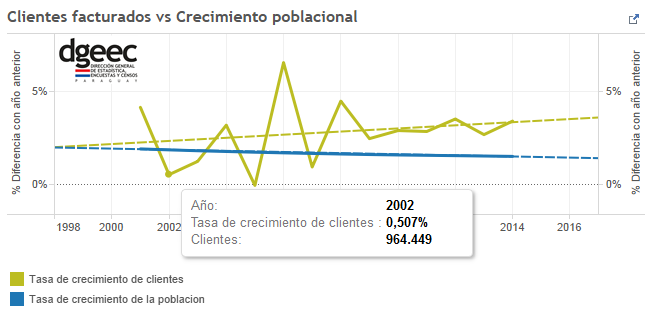
\includegraphics[width=\linewidth]{figuras/ClientesFacturadosVsCrecimientoPoblacional5}
	\caption{Clientes Facturados vs Crecimiento Poblacional}
	\label{fig:ClientesFacturadosVsCrecimientoPoblacional5}
\end{figure}}

\textsc{\begin{figure}[H]
	\centering
	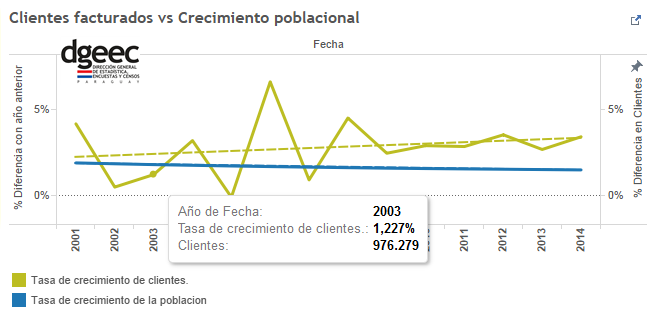
\includegraphics[width=\linewidth]{figuras/ClientesFacturadosVsCrecimientoPoblacional6}
	\caption{Clientes Facturados vs Crecimiento Poblacional}
	\label{fig:ClientesFacturadosVsCrecimientoPoblacional6}
\end{figure}}

En el siguiente gr�fico se realiza una proyecci�n o forecasting donde se muestra que probablemente, si la entidad conserva la misma cantidad de clientes o estos crecen m�nimamente, de igual manera el consumo podr�a aumentar o disminuir dr�sticamente. El aumento dr�stico del consumo, podr�a deberse al aumento de productos electr�nicos que consumen mucha m�s energ�a el�ctrica y tambi�n a que el poder adquisitivo de cada ciudadano ha aumentado. Este comportamiento se observa en la zona de c�lculo de proyecci�n (rojo, azul y amarillo suavizado).



\textsc{\begin{figure}[H]
	\centering
	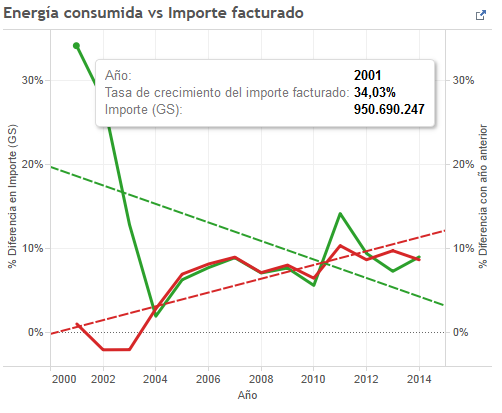
\includegraphics[width=\linewidth]{figuras/EnergiaConsumidaVsImporteFacturado}
	\caption{Energ�a Consumida vs Importe Facturado}
	\label{fig:EnergiaConsumidaVsImporteFacturado}
\end{figure}}

En el tercer y �ltimo gr�fico de este panel, se muestra la porcentaje del crecimiento anual de los importes facturados y consumo de energ�a. Se puede observar que la facturaci�n de la ANDE acompa�a al consumo de energ�a el�ctrica, exceptuando el a�o 2011, en la cual el importe aument� mas de lo que aument� el consumo de energ�a, sin embargo en el a�o 2013 el importe volvi� a aumentar menos que antes.

\textsc{\begin{figure}[H]
	\centering
	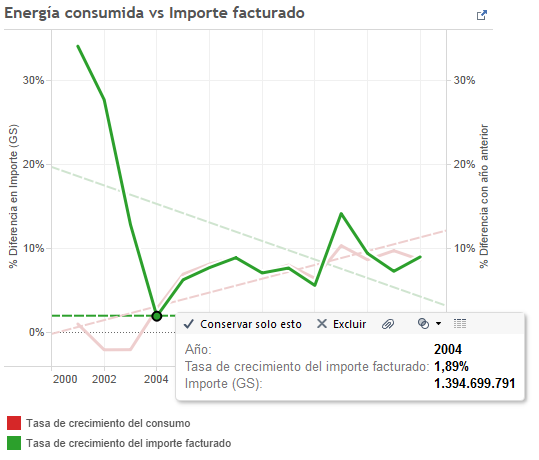
\includegraphics[width=\linewidth]{figuras/EnergiaConsumidaVsImporteFacturado2}
	\caption{Energ�a Consumida vs Importe Facturado}
	\label{fig:EnergiaConsumidaVsImporteFacturado2}
\end{figure}}


\textsc{\begin{figure}[H]
		\centering
		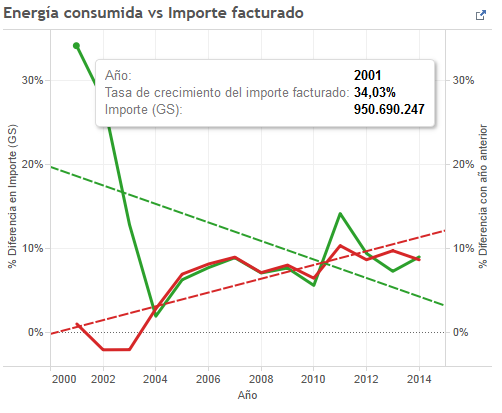
\includegraphics[width=\linewidth]{figuras/EnergiaConsumidaVsImporteFacturado3}
		\caption{Energ�a Consumida vs Importe Facturado}
		\label{fig:EnergiaConsumidaVsImporteFacturado3}
	\end{figure}}
\subsubsection{Panel estad�stico de consumo de electricidad por sector}

En la figura ~\ref{fig:EstadisticaDeConsumoDeElectricidadPorSector1990-2014} se presenta un gr�fico con el consumo de energ�a hist�rica, que abarca desde el a�o 1990 hasta 2014. Estos datos est�n clasificados por los siguientes criterios de la ANDE: Alumbrado P�blico, Comercial, Exportaci�n, Gubernamental, Industrial y Residencial. En este gr�fico se puede apreciar que el mayor consumo de energ�a se encuentra en el sector Residencial. Sin embargo, los valores de Exportaci�n de energ�a fue disminuyendo durante el tiempo. Esto tiene sentido debido a que ambos valores son inversamente proporcionales, esto es, cuando el consumo nacional se incrementa, se hace un mayor uso de energ�a en el pa�s, por lo tanto disminuye la energ�a disponible para exportaci�n.


\textsc{\begin{figure}[H]
	\centering
	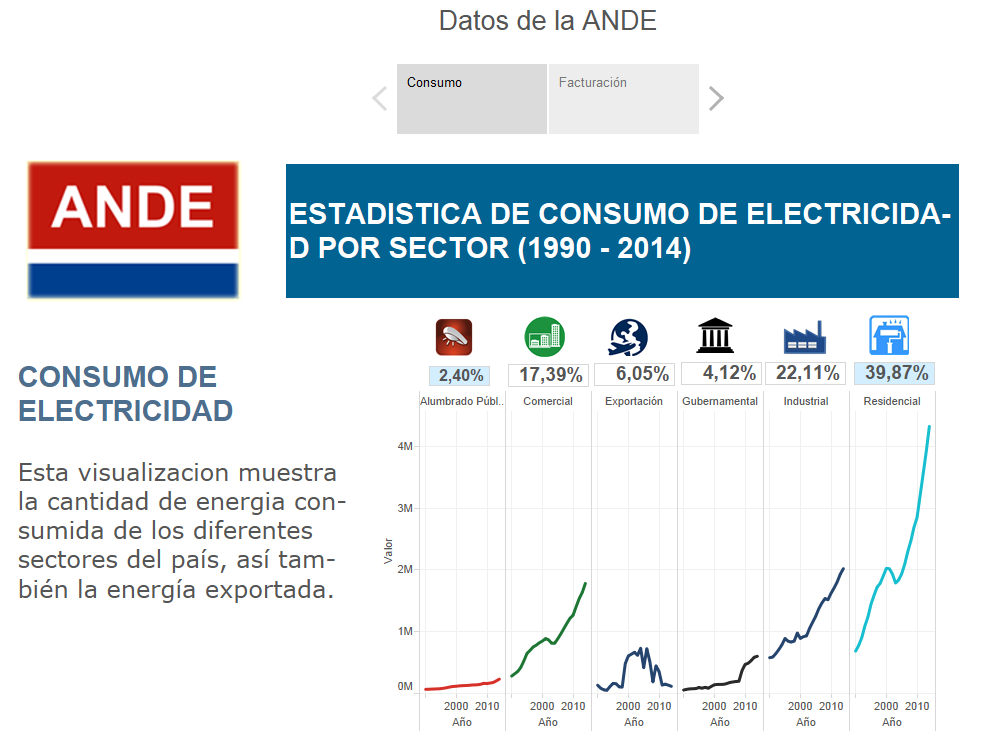
\includegraphics[width=\linewidth]{figuras/EstadisticaDeConsumoDeElectricidadPorSector1990-2014}
	\caption{Estad�stica de consumo de electricidad por sector(1990-2014)}
	\label{fig:EstadisticaDeConsumoDeElectricidadPorSector1990-2014}
\end{figure}}

La Figura ~\ref{fig:ImporteFacturadoPorAnoYSector1990-2014} presenta las informaciones de facturaci�n tambi�n clasificados por sector, con el recurso de filtros por a�o. Es importante destacar un factor resaltante: aunque energ�a exportada disminuy�, el valor facturado por energ�a vendida al exterior aument�. Es probable que esto se haya debido al aumento de la tarifa de energ�a vendida, lo cual beneficia al pa�s.


\textsc{\begin{figure}[H]
	\centering
	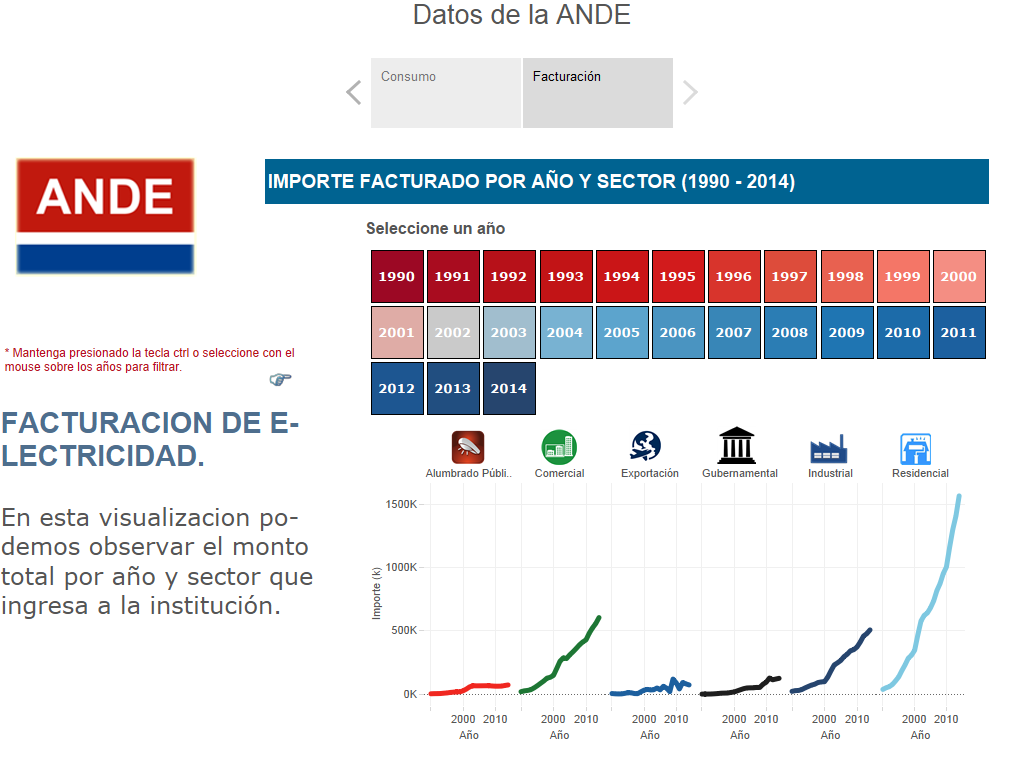
\includegraphics[width=\linewidth]{figuras/ImporteFacturadoPorAnoYSector1990-2014}
	\caption{Importe facturado por a�o y sector(1990-2014)}
	\label{fig:ImporteFacturadoPorAnoYSector1990-2014}
\end{figure}}
\subsubsection{Panel comparativo de Tasa de crecimiento y el Consumo de energ�a}

En la figura ~\ref{fig:TasaDeCrecimientoVsConsumoDeEnergia} se presenta un panel comparativo entre la tasa de crecimiento de clientes y consumo de energ�a. Tambi�n se cuenta con un mapa para filtrar por regi�n del pa�s. 

\textsc{\begin{figure}[H]
	\centering
	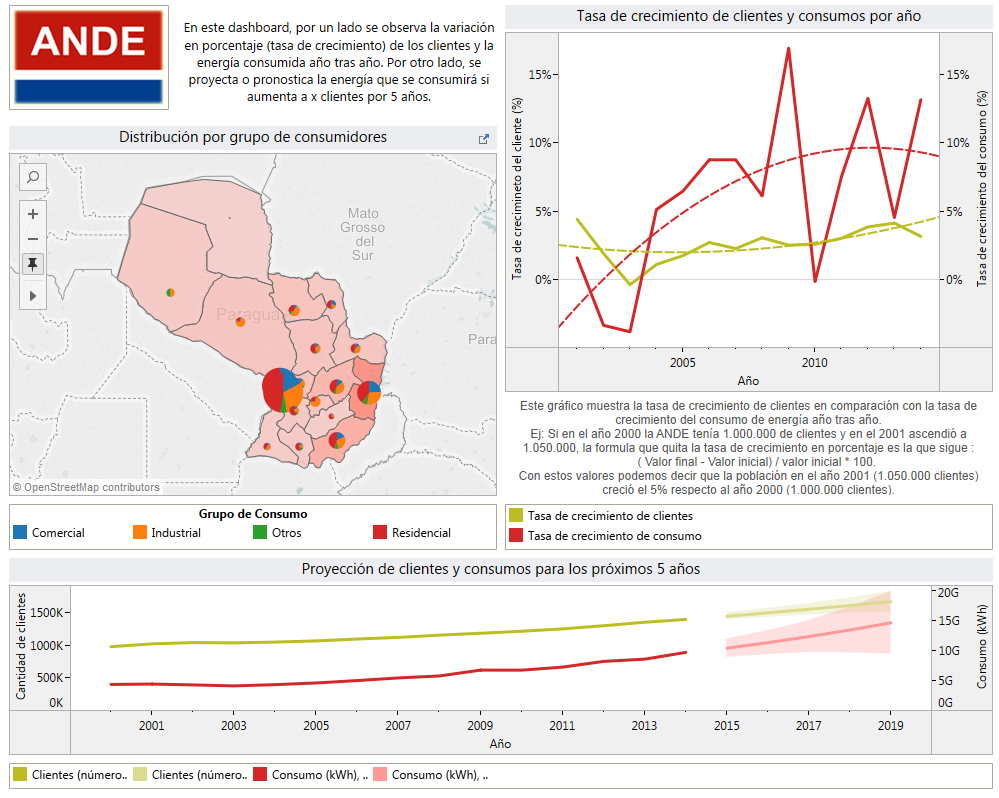
\includegraphics[width=\linewidth]{figuras/TasaDeCrecimientoVsConsumoDeEnergia}
	\caption{Tasa de crecimiento vs Consumo de energ�a}
	\label{fig:TasaDeCrecimientoVsConsumoDeEnergia}
\end{figure}}

En el gr�fico situado a la derecha del mapa (~\ref{fig:TasaDeCrecimientoVsConsumoDeEnergia2}), se tiene el consumo y crecimiento de clientes. Para un mejor analisis fue necesario suavizar los datos calculando lineas de tendencia, debido a una inestabilidad de los datos de consumo. As� se puede apreciar, que existe una tendencia de crecimiento sostenido durante el tiempo de clientes. Sin embargo, la tendencia que el consumo crezca es mayor al de clientes.

\textsc{\begin{figure}[H]
	\centering
	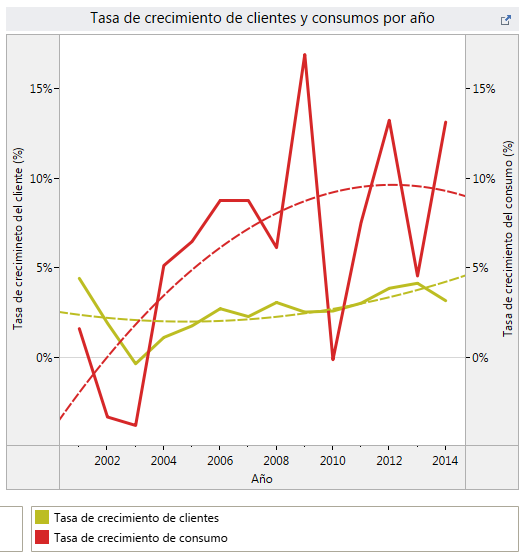
\includegraphics[width=\linewidth]{figuras/TasaDeCrecimientoVsConsumoDeEnergia2}
	\caption{Tasa de crecimiento vs Consumo de energ�a, filtrado por el departamento Alto Paran�}
	\label{fig:TasaDeCrecimientoVsConsumoDeEnergia2}
\end{figure}}

Debajo se presenta un cuadro con la l�nea de cada valor (Figura ~\ref{fig:ProyeccionDeClientesYConsumosParaLosProximos5Anos}), de crecimiento y consumo. Con el uso de un recurso disponible que cuenta la herramienta escogida Tableau, es posible realizar an�lisis predictivo  (forecasting) del crecimiento y consumo. Tableau utiliza un algoritmo llamado Suavizado Exponencial, muy conocido en el �rea de Matem�ticas Estad�sticas. En este gr�fico se puede notar que existe una mayor probabilidad que en los pr�ximos a�os aumente considerablemente el consumo, superando su media. Sin embargo, se nota que el ritmo de crecimiento de clientes es sostenible, y no tiene una alta probabilidad de sufrir un aumento abrupto.

\textsc{\begin{figure}[H]
		\centering
		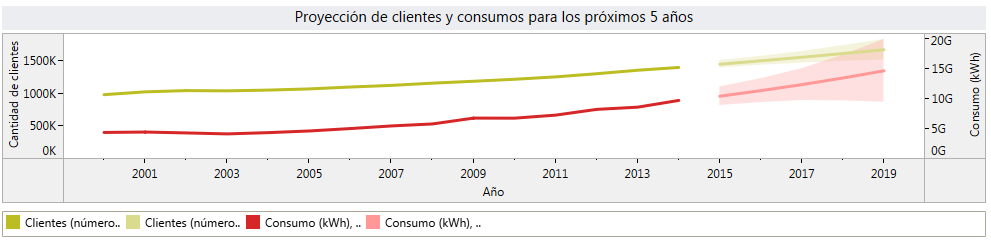
\includegraphics[width=\linewidth]{figuras/ProyeccionDeClientesYConsumosParaLosProximos5Anos}
		\caption{Proyecci�n de clientes y consumos para los pr�ximos 5 a�os}
		\label{fig:ProyeccionDeClientesYConsumosParaLosProximos5Anos}
	\end{figure}}
	
\subsubsection{Dashboard - Tasa de crecimiento poblacional vs Consumo de energ�a a�o tras a�o}

\textsc{\begin{figure}[H]
	\centering
	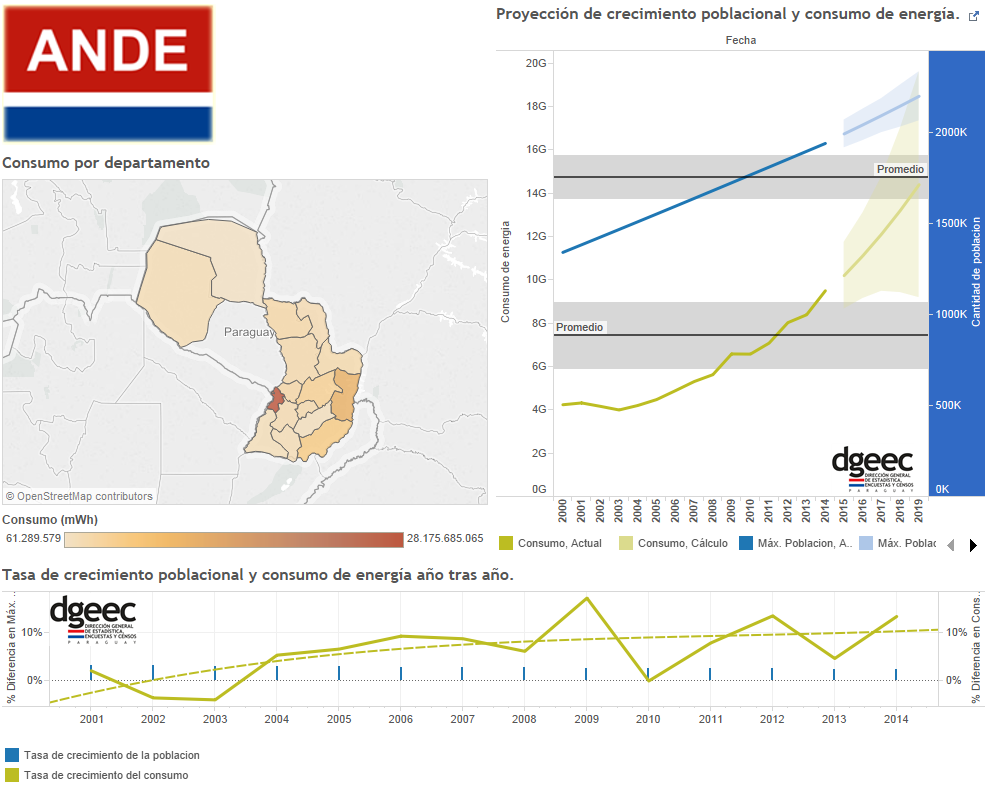
\includegraphics[width=\linewidth]{figuras/TasaDeCrecimientoPoblacionalYConsumoDeEnergiaAnoTrasAno}
	\caption{Dashboard - Tasa de crecimiento poblacional vs consumo de energ�a a�o tras a�o}
	\label{fig:TasaDeCrecimientoPoblacionalYConsumoDeEnergiaAnoTrasAno}
\end{figure}}

En el mapa, donde el color m�s oscuro representa al departamento que consume m�s energ�a el�ctrica y el color m�s claro, al que consume menos, vemos que los departamentos central, Alto Paran� son los que m�s demandan energ�a. Este tipo de gr�fico es muy �til cuando la informaci�n se quiere analizar de forma macro y georeferenciada. Al ubicar el mouse sobre cualquier departamento, se muestra un pop up indicando el valor de consumo del departamento seleccionado. Al dar clic sobre un departamento los dem�s gr�ficos tambi�n se actualizar�n en base a la selecci�n.

\textsc{\begin{figure}[H]
	\centering
	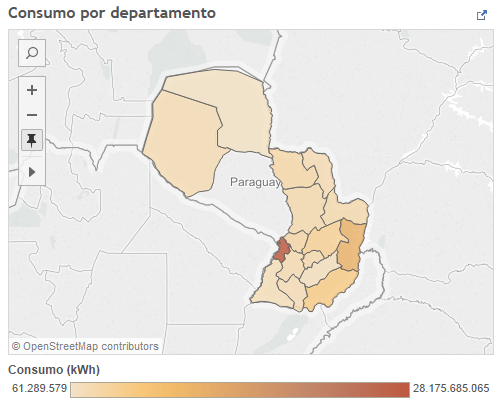
\includegraphics[width=\linewidth]{figuras/TasaDeCrecimientoPoblacionalYConsumoDeEnergiaAnoTrasAnoMapa}
	\caption{Consumo por departamento}
	\label{fig:TasaDeCrecimientoPoblacionalYConsumoDeEnergiaAnoTrasAnoMapa}
\end{figure}}

 En el segundo gr�fico, titulado ``Proyecci�n de crecimiento poblacional y consumo de energ�a``,  vemos el crecimiento de la poblaci�n (n�meros) y el crecimiento del consumo de energ�a el�ctrica expresado en GWh. Al seleccionar un departamento en el mapa, se puede analizar esta informaci�n por cada uno de ellos.


\textsc{\begin{figure}[H]
	\centering
	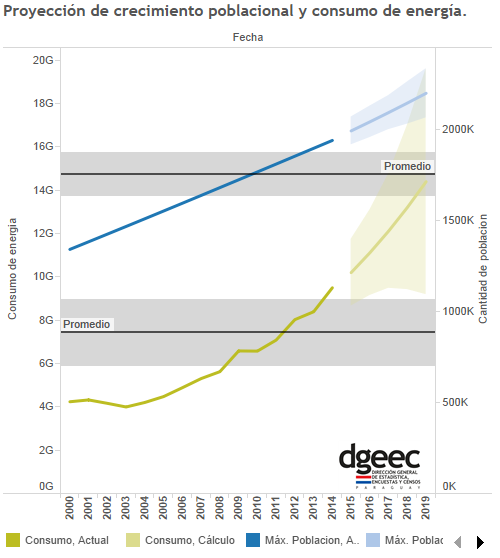
\includegraphics[width=\linewidth]{figuras/ProyeccionDeCrecimientoPoblacionalYConsumoDeEnergia}
	\caption{Proyecci�n de crecimiento poblacional y consumo ee energ�a}
	\label{fig:ProyeccionDeCrecimientoPoblacionalYConsumoDeEnergia}
\end{figure}}

En este gr�fico,  se muestra la misma informaci�n que el gr�fico anterior pero con diferente perspectiva, en este caso se calcula el porcentaje de crecimiento anual tanto de la poblaci�n, as� como del consumo.


\textsc{\begin{figure}[H]
	\centering
	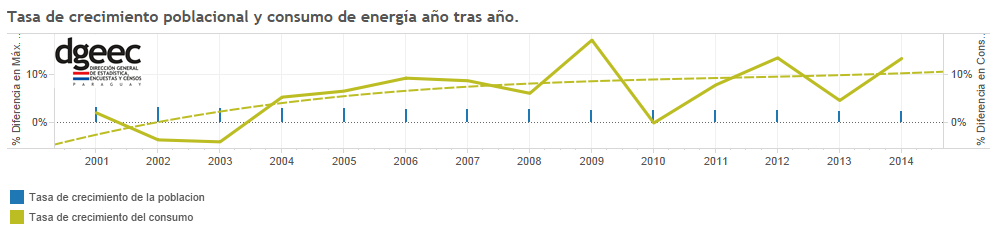
\includegraphics[width=\linewidth]{figuras/ProyeccionDeClientesYConsumosParaLosProximos5Anos2}
	\caption{Tasa de crecimiento poblacional y consumo ee energ�a a�os tras a�os}
	\label{fig:ProyeccionDeClientesYConsumosParaLosProximos5Anos2}
\end{figure}}
